\chapter{IMPLEMENTATION}

\section{System Overview}
The proposed system is an intelligent, self-contained robotic vehicle architecture designed for real-time edge perception, autonomous lane tracking, spatial corridor scanning, and deterministic collision avoidance. The entire system is hosted locally on a Raspberry Pi single-board computer driving an embedded radio-controlled (RC) vehicular chassis without requiring external cloud servers or remote compute nodes.

\begin{figure}[H]
\centering
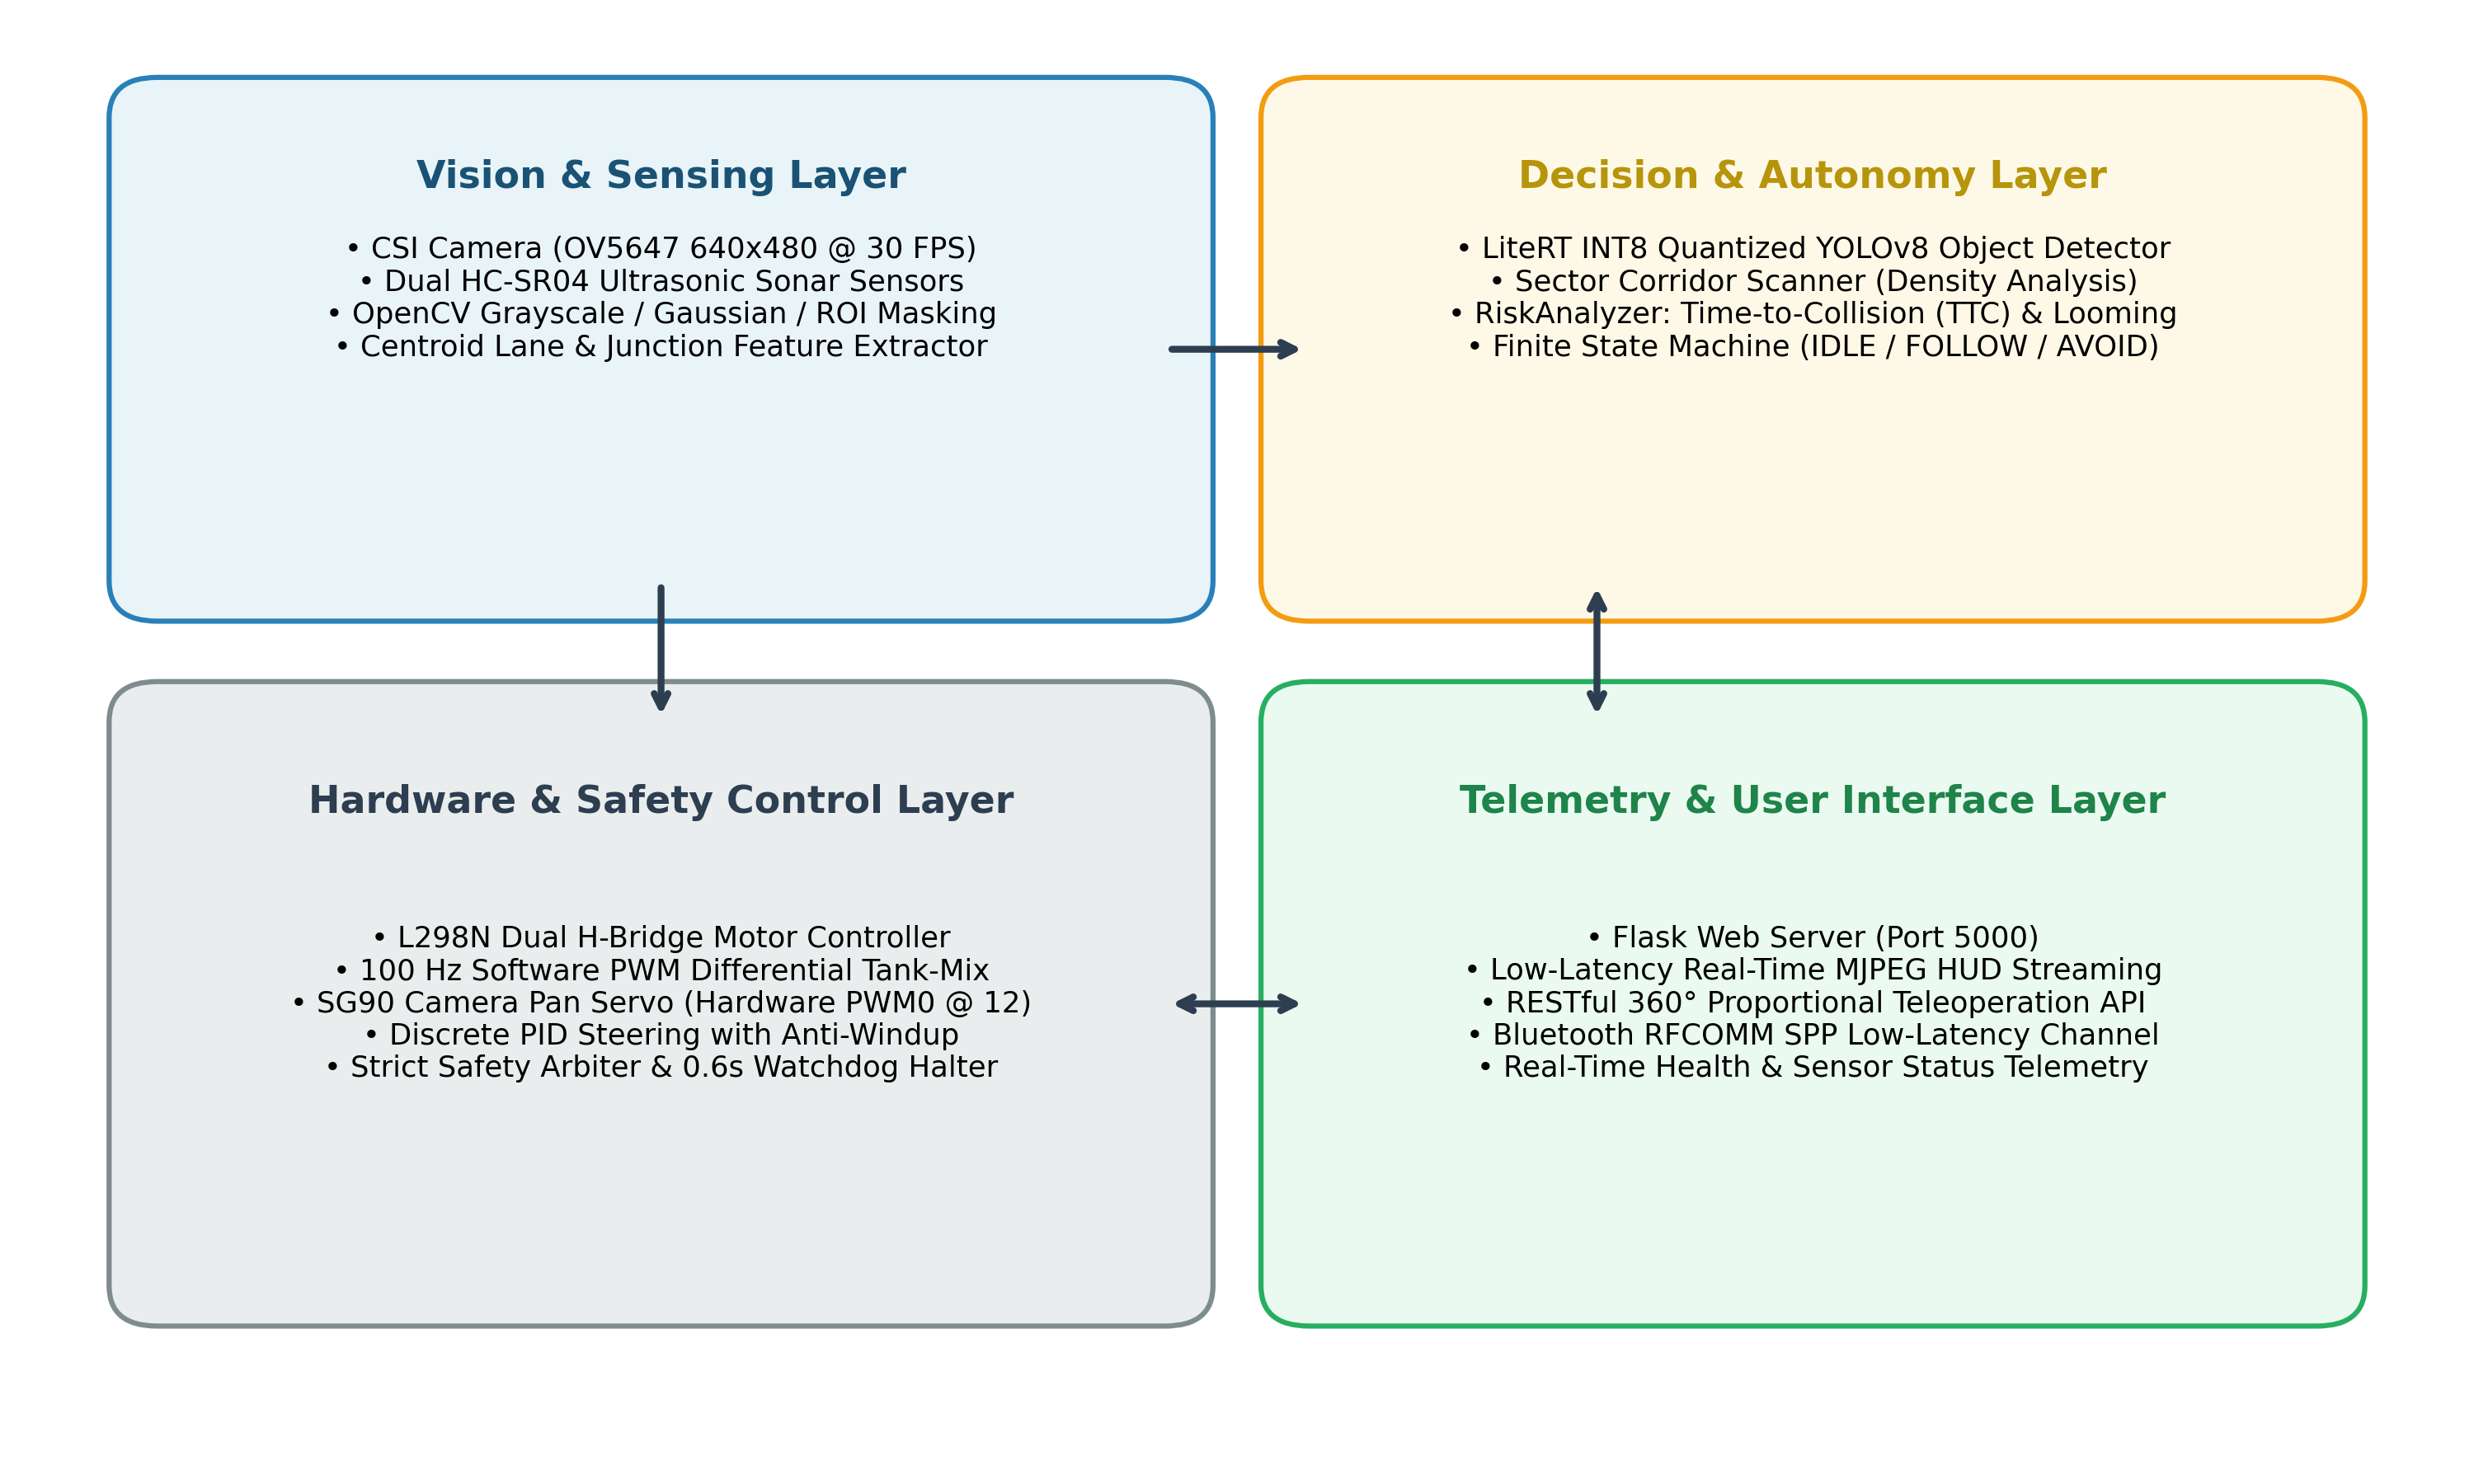
\includegraphics[width=0.92\textwidth]{assets/system_architecture.png}
\caption{Comprehensive Multi-Layer System Architecture of the Autonomous RC Car}
\label{fig:sys_arch}
\end{figure}

As illustrated in Figure~\ref{fig:sys_arch}, the system is organized into four interconnected functional layers:
\begin{enumerate}
    \item \textbf{Vision and Sensing Layer:} Interfacing the physical environment via a high-definition CSI camera (OV5647) executing at 30~FPS, complemented by front and rear ultrasonic distance sensors (HC-SR04).
    \item \textbf{Decision and Autonomy Layer:} Implementing high-speed computer vision preprocessing, INT8-quantized YOLOv8 object detection via Google LiteRT, spatial corridor density clearance analysis, and a thread-safe Finite State Machine (FSM).
    \item \textbf{Hardware and Safety Control Layer:} Coordinating an L298N dual H-bridge motor driver over 100~Hz software Pulse Width Modulation (PWM), an SG90 camera survey pan servo over dedicated hardware PWM0 on GPIO 12, a discrete PID steering regulator, and a strict safety arbiter.
    \item \textbf{Telemetry and User Interface Layer:} Hosting an asynchronous Flask web server on port 5000, streaming low-latency MJPEG video with real-time Heads-Up Display (HUD) overlays, providing 360-degree proportional joystick teleoperation, and maintaining a secondary Bluetooth RFCOMM serial channel.
\end{enumerate}

\section{Hardware and Software Specifications}
The physical platform is constructed using modular, industry-standard robotics components configured for maximum thermal and computational efficiency. Table~\ref{tab:hardware_spec} outlines the core hardware specifications of the autonomous vehicle.

\begin{table}[H]
\caption{System Hardware and Sensor Specifications}
\label{tab:hardware_spec}
\begin{center}
\resizebox{0.95\columnwidth}{!}{
\begin{tabular}{|l|l|l|}
\hline
\textbf{Subsystem} & \textbf{Component / Module} & \textbf{Technical Specification / Role} \\
\hline
Single-Board Computer & Raspberry Pi 3/4 & 64-bit Quad-Core ARM Cortex-A72 CPU, Linux OS \\
Primary Vision Sensor & OV5647 CSI Camera Module & 5 Megapixel, 15-pin CSI bus, 640$\times$480 @ 30 FPS \\
Ranging Sensors & Dual HC-SR04 Ultrasonic & 40 kHz acoustic ping, 2 cm to 400 cm range ($\pm 3$ mm) \\
Motor Driver & L298N Dual H-Bridge & Dual full-bridge driver, 2A peak per channel, heat-sinked \\
Steering / Pan Actuator & SG90 Micro Servo & 50 Hz PWM, 180$^\circ$ sweep, hardware PWM0 on GPIO 12 \\
Drive Motors & 4$\times$ DC Gearmotors & Differential drive configuration, 6V operating voltage \\
Power Source & Dual Power Architecture & 7.4V 2S LiPo (Motors) + 5V/3A DC Buck Converter (Pi) \\
Wireless Interconnect & On-board Wi-Fi \& Bluetooth 5.0 & 2.4/5 GHz 802.11ac + RFCOMM Bluetooth SPP channel \\
\hline
\end{tabular}
}
\end{center}
\end{table}

\subsection{Electrical Wiring and GPIO Pinout Mapping}
To prevent electrical noise from the high-current DC motors from interfering with the sensitive digital logic of the Raspberry Pi, a strict star-topology common ground is maintained between the battery, L298N logic ground, and Raspberry Pi digital ground pins. Furthermore, because the HC-SR04 ultrasonic echo pulse outputs a 5.0~V TTL logic signal that exceeds the 3.3~V maximum tolerance of the Raspberry Pi GPIO pins, a passive resistor voltage divider (1~k$\Omega$ and 2~k$\Omega$) is integrated to step the echo pulse down to 3.3~V safely. Table~\ref{tab:pin_mapping} details the pin assignments.

\begin{table}[H]
\caption{Raspberry Pi BCM GPIO Pin Allocation and Electrical Interconnect}
\label{tab:pin_mapping}
\begin{center}
\resizebox{0.95\columnwidth}{!}{
\begin{tabular}{|l|l|l|l|}
\hline
\textbf{Physical Function} & \textbf{BCM GPIO} & \textbf{Physical Header Pin} & \textbf{Signal Electrical Characteristics} \\
\hline
Left Motor Forward / PWM & GPIO 17 & Pin 11 & Software PWM, 100 Hz, 3.3V Logic \\
Left Motor Reverse / PWM & GPIO 27 & Pin 13 & Primary Left Motor Reverse Signal \\
Left Motor Alternate Mirror & GPIO 18 & Pin 12 & Automatic dual-drive auto-mirror fallback \\
Right Motor Forward / PWM & GPIO 22 & Pin 15 & Software PWM, 100 Hz, 3.3V Logic \\
Right Motor Reverse / PWM & GPIO 23 & Pin 16 & Software PWM, 100 Hz, 3.3V Logic \\
Camera Pan Servo & GPIO 12 & Pin 32 & Hardware PWM0, 50 Hz (20 ms period), 0--180$^\circ$ \\
Front Sonar Trigger & GPIO 24 & Pin 18 & 10 $\mu$s digital pulse trigger output \\
Front Sonar Echo & GPIO 25 & Pin 22 & 3.3V scaled input via 1k$\Omega$/2k$\Omega$ divider \\
Digital System Ground & GND & Pin 6 / Pin 9 & Common logic ground tied to L298N GND \\
\hline
\end{tabular}
}
\end{center}
\end{table}

\subsection{Software Stack and Frameworks}
The software architecture is implemented in Python running on 64-bit Debian GNU/Linux:
\begin{itemize}
    \item \textbf{Image Acquisition:} Native \texttt{Picamera2} library providing asynchronous, zero-copy memory buffer frame capture directly from the camera sensor pipeline.
    \item \textbf{Computer Vision:} \texttt{OpenCV} (v4.x) for color space transformation, Gaussian blur filtering, adaptive binary thresholding, morphological closing (\texttt{MORPH\_CLOSE}), and polygonal ROI mask generation.
    \item \textbf{Edge Machine Learning:} \texttt{ai\_edge\_litert} runtime executing INT8-quantized YOLOv8 Nano weights with letterbox aspect-ratio preservation.
    \item \textbf{Hardware Abstraction:} \texttt{RPi.GPIO} controlling software PWM channels at 100~Hz for motor velocity modulation and hardware PWM timing on GPIO 12 for servo survey.
    \item \textbf{Web Framework:} \texttt{Flask} microframework serving asynchronous RESTful driving endpoints and multipart MJPEG stream encoding with low-overhead HTTP response generation.
\end{itemize}

\section{System Workflow}
The continuous operational cycle of the autonomous vehicle executes along a deterministic closed-loop pipeline at approximately 30~Hz, as diagrammed in Figure~\ref{fig:workflow_pipe}.

\begin{figure}[H]
\centering
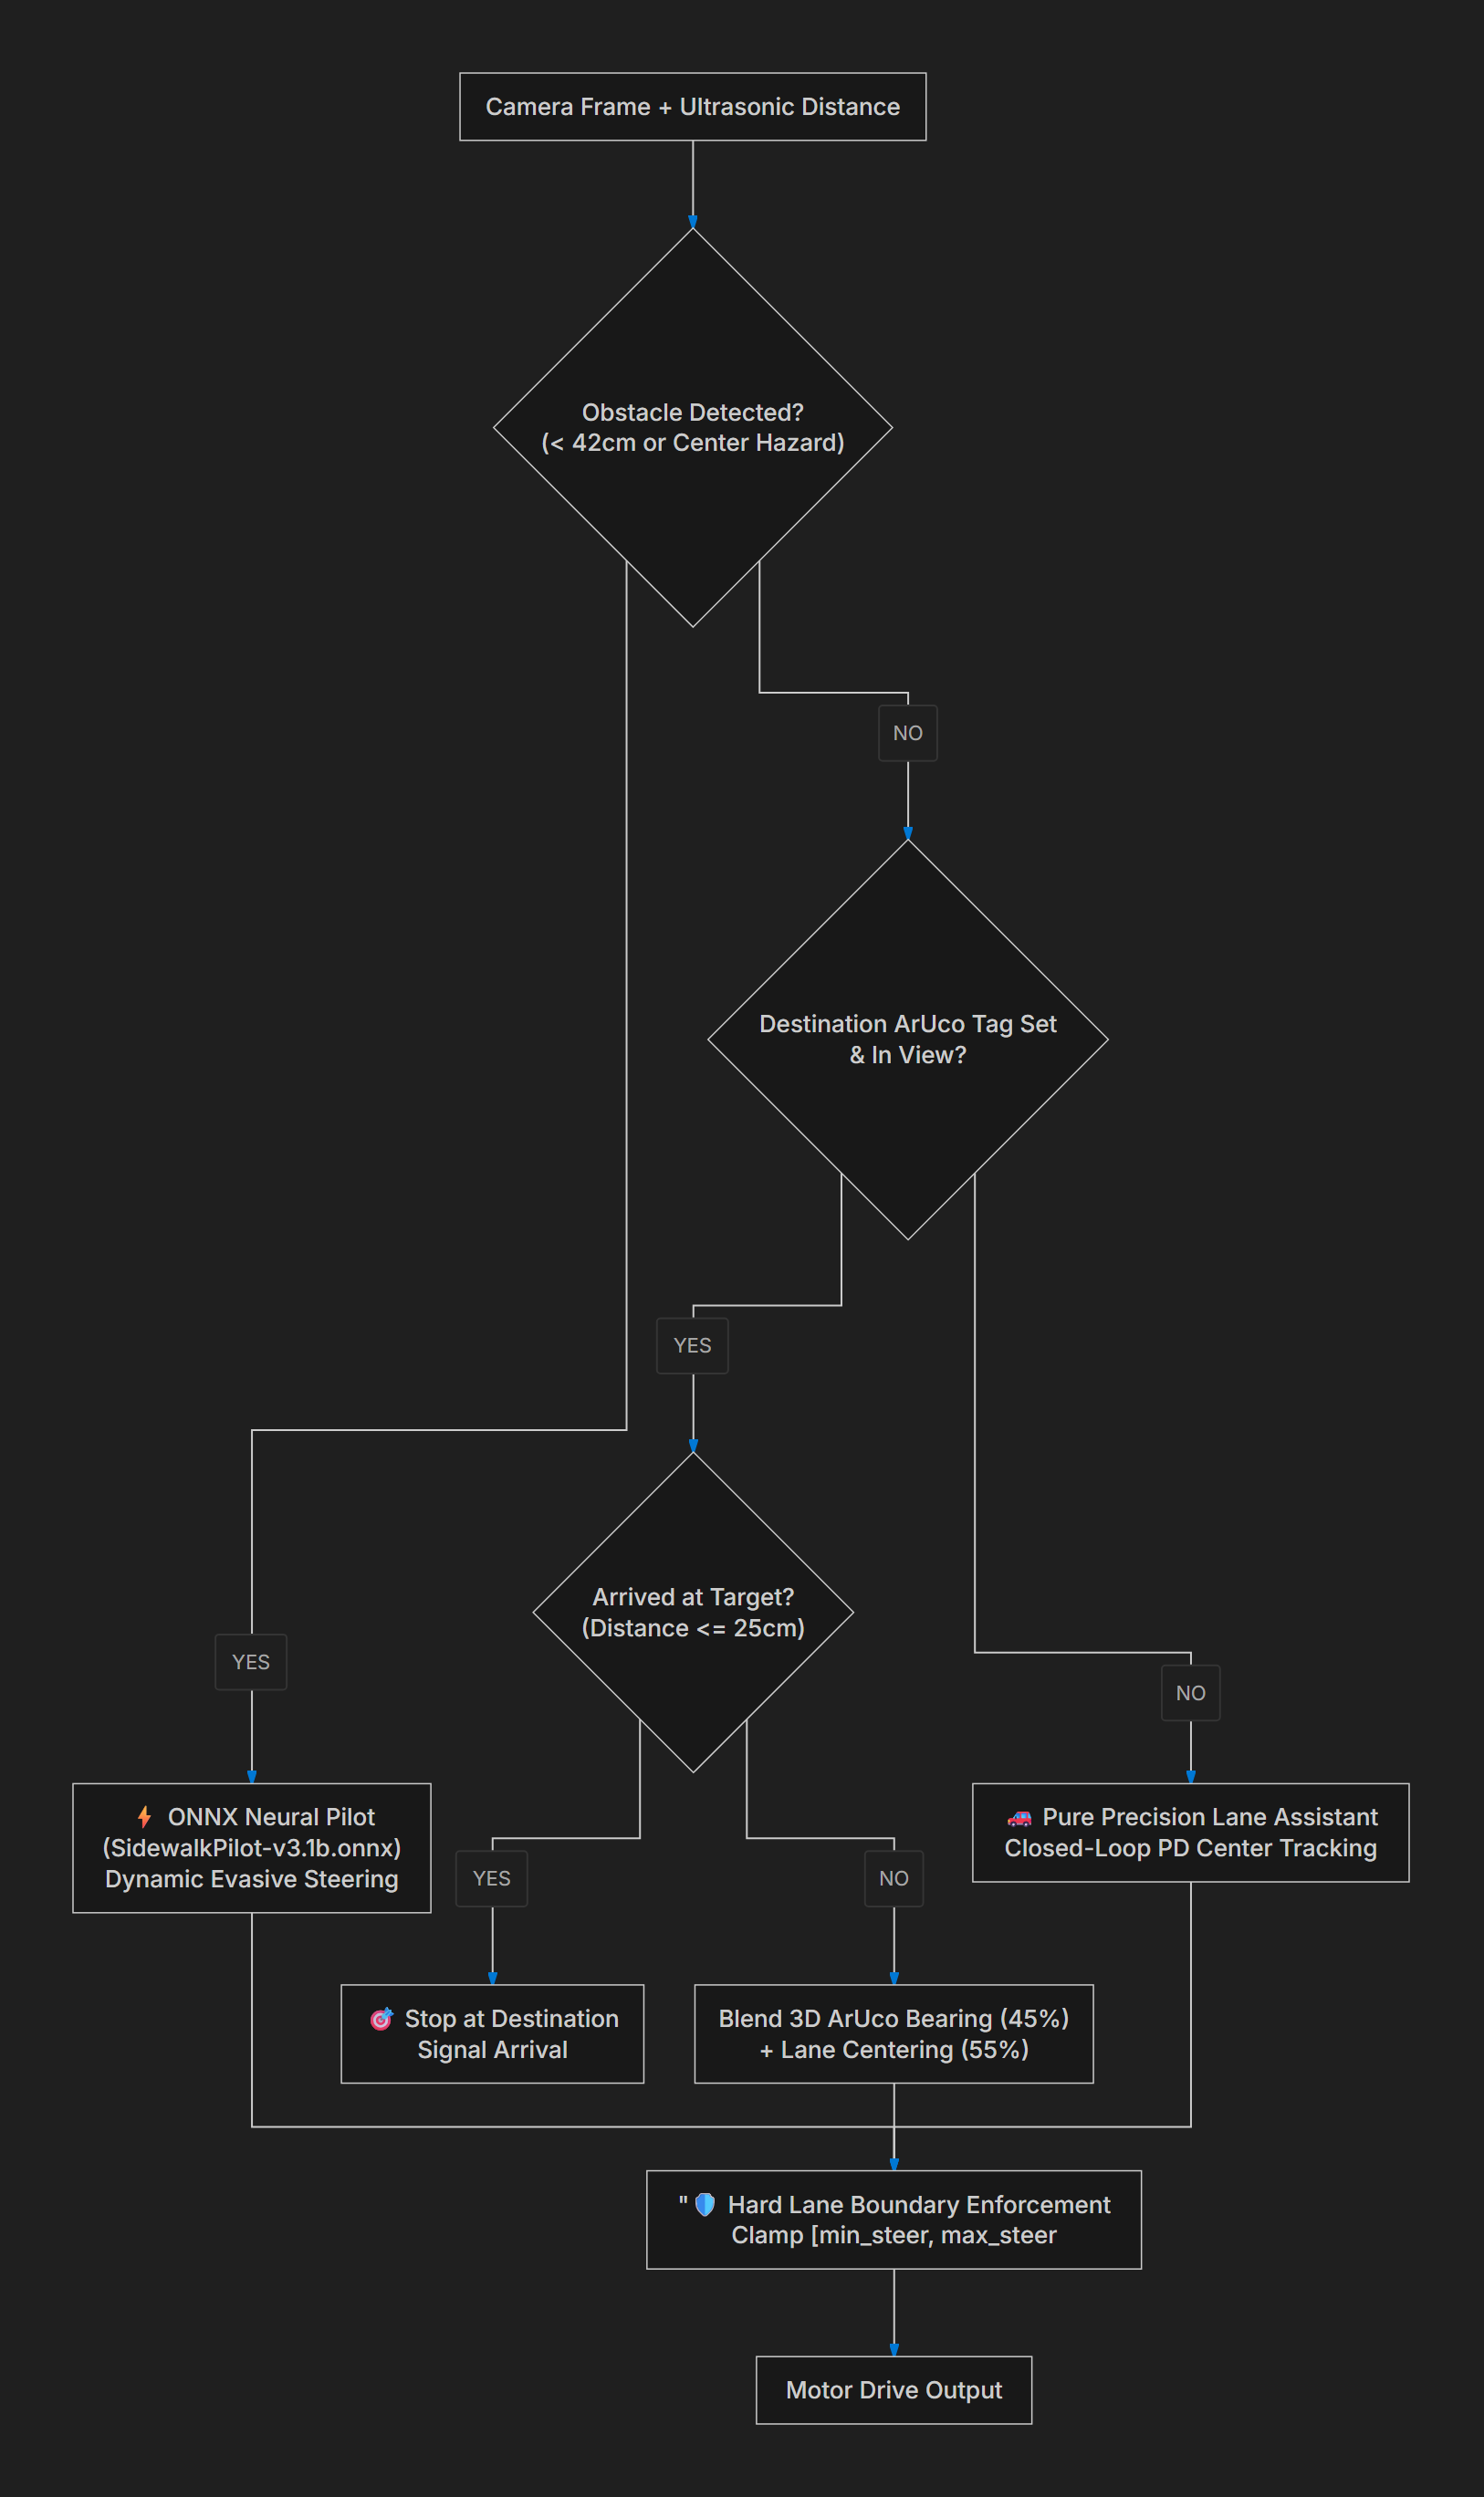
\includegraphics[width=0.95\textwidth]{assets/system_workflow.png}
\caption{End-to-End Operational Execution Pipeline and Feedback Loop}
\label{fig:workflow_pipe}
\end{figure}

The execution sequence proceeds through five synchronized stages:
\begin{enumerate}
    \item \textbf{Perception Capture:} The camera background thread retrieves a 640$\times$480 BGR frame while the ultrasonic thread emits a 10~$\mu$s trigger pulse on GPIO 24, measuring the return echo width $\Delta t$ on GPIO 25 to compute the obstacle distance $d = \frac{\Delta t \cdot 34300}{2}$~cm.
    \item \textbf{Computer Vision Processing:} The captured image is cropped to a trapezoidal Region of Interest (the lower 55\% of the frame). The system computes the binary centroid error $e = C_x - \frac{W}{2}$.
    \item \textbf{Edge AI and Corridor Analysis:} The image is passed to the LiteRT YOLOv8n INT8 interpreter to identify semantic objects (pedestrians, vehicles, stop signs). Concurrently, the Corridor Scanner splits the foreground into Left, Center, and Right sectors, evaluating gradient density to calculate clear path vectors.
    \item \textbf{Motion Planning and State Machine:} A discrete PID controller calculates the required steering correction $u(t) = K_p e(t) + K_i \int e(t) dt + K_d \frac{de(t)}{dt}$. The Finite State Machine transitions between states (\texttt{IDLE}, \texttt{FOLLOW\_LANE}, \texttt{OBSTACLE}, \texttt{SCANNING}) based on fused sensor confidence.
    \item \textbf{Safety Arbiter and Actuation:} The motion command is passed to the Safety Arbiter. If front sonar detects an obstacle under 15~cm or the watchdog timer exceeds 0.6 seconds without a fresh valid reading, the arbiter overrides the planner and forces instantaneous motor braking ($u = 0, \text{throttle} = 0$).
\end{enumerate}

\section{Kinematic Differential Drive and Motor Modulation}
Vehicle maneuvering is governed by differential drive kinematics. Left and right wheel PWM duty cycles are calculated using a 360-degree proportional tank-mixing algorithm:
\begin{equation}
V_{\text{left}} = \text{throttle} + \text{steering}, \quad V_{\text{right}} = \text{throttle} - \text{steering}
\end{equation}
The computed velocities are clamped to $[-1.0, 1.0]$ and scaled against persistent calibration trims to compensate for physical motor manufacturing variances:
\begin{equation}
\text{PWM}_{\text{left}} = \max(-100, \min(100, V_{\text{left}} \cdot \text{trim}_{\text{left}} \cdot 100))
\end{equation}
\begin{equation}
\text{PWM}_{\text{right}} = \max(-100, \min(100, V_{\text{right}} \cdot \text{trim}_{\text{right}} \cdot 100))
\end{equation}
To eliminate physical wiring discrepancies where GPIO 18 and GPIO 27 are interchangeably wired across revisions, the motor controller automatically mirrors the reverse PWM signal across both pins, ensuring reliable operation under all hardware configurations.
